\chapter{Teoretične osnove}

Energetske parametre za izbrani odsek vodotoka lahko izračunamo po naslednjem algoritmu:
\begin{enumerate}[noitemsep, topsep=0pt]
	\item Pridobitev podatkov
	\item Analiza hidrološkega niza podatkov za iskano obdobje
	\item Izračun konsumpcijske krivulje
	\item Izračun povprečne letne proizvodnje električne energije
\end{enumerate}


%-------------------------------------
\section{Pridobitev podatkov} \label{sec:teorija_pridobitevPodatkov}
Za nadaljnje izračune potrebujemo podatke o:
\begin{itemize}[noitemsep, topsep=0pt]
	\item Geometriji in naklonu rečne struge
	\item Manningovem koeficientu hrapavosti rečnega korita
	\item Povprečnih dnevnih pretokih vodotoka za izbrano obdobje
\end{itemize}


Podatke o geometriji rečnega korita lahko pridobimo iz javne baze podatkov (npr. LIDAR, ortofoto), praviloma pa je treba natančnejše posnetke zagotoviti z geodetskimi meritvami na terenu. Za potrebe ocene hidroenergetskega potenciala niso potrebne natančne izmere, zato smo geometrijo struge določili na podlagi ortofoto posnetkov. Naklon rečne struge vodotoka se lahko oceni s pomočjo spletne aplikacije Geopedija. Na karti v spletni aplikaciji Geopedija si izberemo dve točki, ki definirata odsek analiziranega vodotoka in odčitamo podatke o višinski razliki $\Delta h$ in razdalji $\Delta L$ med izbranima točkama. S pomočjo spodnje enačbe določimo naklon izbranega odseka vodotoka:


%BEFORE:
%Podatke o dimenzijah rečnega korita lahko pridobimo z meritvami na terenu ali pa dimenzije ocenimo na podlagi ortofoto posnetkov. Naklon rečne struge vodotoka se lahko oceni s pomočjo spletne aplikacije Geopedija. Na karti v spletni aplikaciji Geopedija si izberemo dve točki, ki definirata odsek analiziranega vodotoka in odčitamo podatke o višinski razliki $\Delta h$ in razdalji $\Delta L$ med izbranima točkama. S pomočjo spodnje enačbe določimo naklon izbranega odseka vodotoka:

\begin{ceqn}
\begin{align}
 I = \dfrac{100\Delta h}{\Delta L} [\%]
\end{align}
\end{ceqn}


  Manningov koeficient hrapavosti rečnega korita $ng$ se lahko oceni izkustveno na terenu s pomočjo priročnikov ali pa z umerjanjem na podlagi podatkov o nivojih vode in pretokih. Manningov koeficient hrapavosti $ng$ je odvisen od naslednjih 7 faktorjev \cite{VenTeChow}:
 \begin{enumerate}[noitemsep, topsep=0pt]
 	\item Hrapavosti površine ostenja
 	\item Zaraščenosti rečnega korita
 	\item Neregularnosti oblike rečnega korita
 	\item Meandriranja rečne struge
 	\item Zamašitve struge s plavinami 
 	\item Oblike in velikosti rečnega korita
 	\item Polnosti rečnega korita z vodo
 \end{enumerate}
 

 
 
  Podatke o pretokih slovenskih vodotokov lahko pridobimo iz arhiva, ki se nahaja na spletni strani agencije Republike Slovenije za okolje (v nadaljevanju ARSO). V primeru da iščemo pretok za manjši vodotok, je zelo verjetno da podatki o pretokih vodotoka ne obstajajo. V tem primeru lahko pretok vodotoka ocenimo s pomočjo meritev višine gladine vode in dimenzij struge, ocene Manningovega koeficienta hrapavosti in naklona struge. S pomočjo Manningove enačbe opisane kasneje v poglavju~\ref{sec:teorija_trapeznaMetoda} dobimo končno ocenjeno vrednost pretoka vodotoka za posamezno obdobje meritev.




%------------------------------------------------
\section{Analiza hidrološkega niza podatkov}~\label{sec:teorija_hidrogramObdobja}
Namen analize hidrološkega niza podatkov je priprava podatkov za nadaljnje izračune energetskih parametrov hidroelektrarne. Potrebovali bomo hidrogram obdobja in krivuljo trajanja. Hidrogram obdobja je diagram, ki prikazuje povprečne mesečne pretoke vodotoka za izbrano obdobje analize vodotoka, sortirane v kronološkem vrstnem redu. S pomočjo hidrograma lahko ocenimo rečni režim našega vodotoka in nihanja vrednosti povprečnih mesečnih pretokov vodotoka skozi leto. Po navadi na hidrogramu tudi prikažemo vrednosti pretokov za mokro in suho leto, t.j. leto z maksimalnimi oz. minimalnimi vrednostmi pretokov vodotoka v izbranem obdobju analize. S tem ponazorimo nihanje pretokov vodotoka, ki se lahko pojavi v bodočem času obratovanja hidroelektrarne.


Krivulja trajanja je diagram, ki prikazuje podatke iz hidrograma, t.j. povprečne mesečne pretoke vodotoka v analiziranem obdobju sortirane po vrsti padajoče. S pomočjo krivulje trajanja si ponazorimo čas trajanja posameznih vrednosti pretokov izbranega vodotoka. Poleg tega si s krivuljo trajanja pomagamo pri izbiri ustrezne vrste in velikosti turbin v času načrtovanja hidroelektrarne.


%------------------------------------------------
\section{Izračun konsumpcijske krivulje}
Konsumpcijska krivulja je graf funkcije, ki predstavlja višino gladine vode v odvisnosti od pretoka vode v rečni strugi. Graf konsumpcijske krivulje potrebujemo za določitev višinske razlike $dh$ med spodnjo in zgornjo vodo hidroelektrarne v odvisnosti od pretoka vode skozi turbine hidroelektrarne. Višinsko razliko $dh$ potrebujemo za določitev moči hidroelektrarne in izračun proizvedene električne energije. Postopek za izračun navedenega je opisan v zadnjem koraku algoritma za izračun energetskih parametrov hidroelektrarne v tem poglavju.



%-------------------------------------------------
\subsection{Izračun konsumpcijske krivulje za pravokotne in trapezne struge} \label{sec:teorija_trapeznaMetoda}
Za izris konsumpcijske krivulje potrebujemo vrednosti pretoka vodotoka $Q$ v odvisnosti od višine gladine vode $h$ v rečni strugi. Gladina vode $h$ poteka od najnižje točke v strugi do maksimalne višine gladine vode v strugi vodotoka $H$. Natančnost rezultatov numeričnih metod, je odvisna od velikosti koraka izračuna. V našem primeru za potrebe ocene pretoka, centimetrski korak po višini predstavlja zadostno natančnost. Pretok vode v odprti strugi $Q$ se torej za vsak cm višine $h$ izračuna po Manningovi enačbi: 

\begin{ceqn}
\begin{align}
Q = \dfrac{\sqrt{I}}{ng} \cdot S \cdot R^{2/3} \label{eq:ManningovaEnacba}
\end{align}
\end{ceqn}


Kjer je:
\begin{table}[H]
	\begin{tabular}{r|p{10cm}}
		Q & pretok \\
		ng & Manningov koeficient hrapavosti dna struge\\
		I & naklon struge \\
		S & ploščina dela prečnega profila pod gladino vode\\
		R & hidravlični radij $\dfrac{S}{P}$\\
		P & dolžina omočenega oboda struge\\
	\end{tabular}
\end{table}

Če člene Manningove enačbe izpišemo dobimo spodnjo enačbo:

\begin{ceqn}
	\begin{align}
	Q(h) = \dfrac{\sqrt{I}}{ng} \cdot \dfrac{S(h)^{5/3}}{P(h)^{2/3}} \label{eq:ManningovaEnacba}
	\end{align}
\end{ceqn}


Dobili smo končno enačbo katero bomo uporabljali v nadaljevanju pri izračunu pretokov po višini za pravokotne in trapezno oblikovane struge.



% pravokotna struga
\begin{enumerate}
	\item Pravokotno oblikovana struga vodotoka:
	
	\begin{figure}[H]
		\begin{centering}
			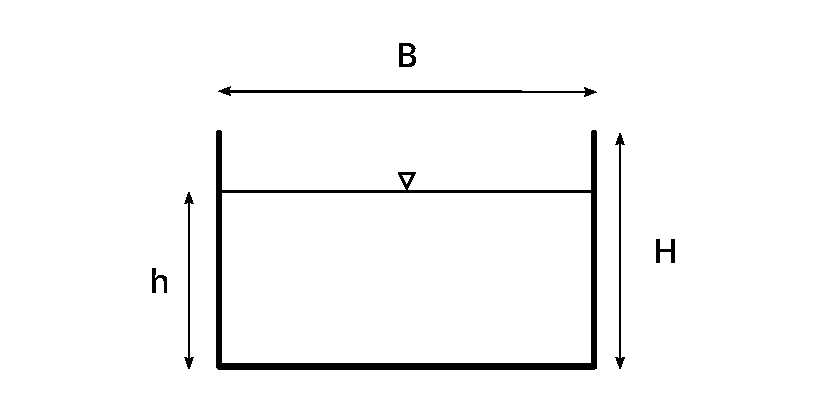
\includegraphics{slike/konsumpcijska_krivulja/rectangularChannel.pdf}		
			\caption{Prečni prerez pravokotne struge}\label{fig:pravokotna struga}
		\end{centering}
	\end{figure}
	

	Omočeni obod pravokotno oblikovane struge $P_p(h)$ izračunamo kot seštevek širine struge $B$ in dvakratne višine gladine vode v rečnem koritu $h$:
	
	\begin{ceqn}
	\begin{equation}
	P_{p}(h) = B + 2h
	\end{equation}
	\end{ceqn}
	
	Ploščino prečnega prereza struge vodotoka pod gladino vode $S_p(h)$ za pravokotno oblikovano strugo dobimo po enačbi:
	
	\begin{ceqn}
	\begin{align}
	S_{p}(h) = B \cdot h
	\end{align}
	\end{ceqn}
	
	\item Trapezno oblikovana struga vodotoka:
	
		\begin{figure}[ht!]
			\begin{centering}
				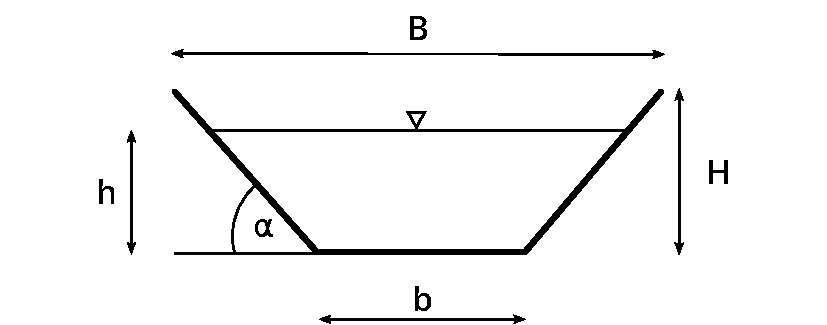
\includegraphics{slike/konsumpcijska_krivulja/trapezoidChannel.pdf}		
				\caption{Prečni prerez trapezne struge}\label{fig:trapezna struga}
			\end{centering}
		\end{figure}
	
	Omočeni obod trapezno oblikovanega rečnega korita $P_t(h)$ izračunamo kot seštevek širine dna struge in dvakratne razdalje od roba dna do točke presečišča rečnega korita z gladino vode:
	
	\begin{ceqn}
	\begin{align}
	P_{t}(h) = b + 2 \cdot \sqrt{h^2 + \left(\dfrac{h} {\tan\alpha} \right)^{2}}
	\end{align}
	\end{ceqn}
	
	Ploščino prečnega prereza struge pod gladino vode $S_t(h)$ za trapezno oblikovano rečno korito izračunamo po enačbi:
	\begin{ceqn}
	\begin{align}
	S_{t}(h) = b \cdot h + \dfrac{h^2}{\tan\alpha}
	\end{align}
	\end{ceqn}
	
\end{enumerate}



Ko poznamo vse člene Manningove enačbe \ref{eq:ManningovaEnacba}, izračunamo pretoke vodotoka za vsak cm višine gladine vode v rečni strugi, ki poteka od višine $h=0$ do višine $h=H$. S tem smo izračunali točke diagrama konsumpcijske krivulje $h(Q)$. S pomočjo konsumpcijske krivulje bomo v naslednjih poglavjih določali višino spodnje vode hidroelektrarne v rečni strugi.



%------------------------------------------------
\subsection{Izračun konsumpcijske krivulje za struge poljubne oblike} \label{sec:teorija_metodaPoljubnaOblika}


V primeru, da iščemo konsumpcijsko krivuljo za strugo vodotoka poljubne oblike, si za izračun členov Manningove enačbe ($S(h)$ in $P(h)$) ne moremo pomagati z znanimi formulami preprostih geometrijskih likov. Poljubno oblikovano strugo lahko modeliramo s serijo točk, ki jih dodajamo v kartezijski koordinatni sistem $x,y$. Za vsako točko ki definira poljubno rečno korito podamo x in y koordinato, za točke pa predpostavimo, da so med seboj povezane z enačbo linearne funkcije. Na sliki~\ref{fig:poljubnaStruga} je predstavljena shema prečnega prereza poljubno oblikovane struge vodotoka.

\begin{figure}[ht!]
	\begin{centering}
		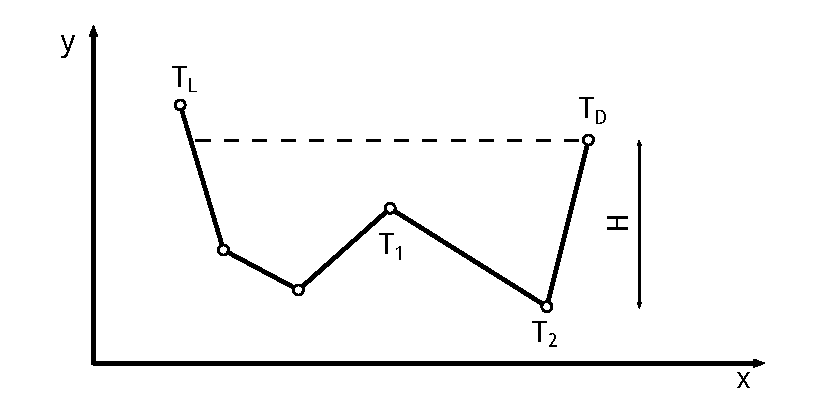
\includegraphics{slike/customChannel/customStruga.pdf}\caption{Prečni prerez poljubno oblikovane struge vodotoka}\label{fig:poljubnaStruga}
	\end{centering}
\end{figure}



%------------------------------------------
%\subsection{Izračun višine rečnega korita}
Skrajni točki na robu struge vodotoka sta točki $T_L$ in $T_D$ prikazani na sliki \ref{fig:poljubnaStruga}. Točko na robu struge z nižjo y koordinato označimo s $T_{Rmin}$ (na sliki \ref{fig:poljubnaStruga} desna skrajna točka označena kot točka $T_D$). Najnižjo točko struge vodotoka označimo s $T_{min}$. Maksimalna višina gladine vode v rečnem koritu $H$ je definirana kot razdalja med točkama $T_{Rmin}$ in $T_{min}$. Obilno deževje, ki privede do poplav, lahko povzroči, da bi bil pretok vodotoka večji od pretoka, ki ga je rečno korito sploh sposobno prevajati. V tem primeru se voda začne prelivati preko robov struge vodotoka, višina gladine vode v strugi pa je zaradi preliva vode preko robov vodotoka še vedno enaka maksimalni višini gladine $h=H$.



%\subsection{Določitev parametrov odseka}
Za izračun konsumpcijske krivulje, s točkami definirano poljubno strugo vodotoka najprej razdelimo na $n$ odsekov po dve točki $O_1$ ($x_1$, $y_1$) in $O_2$ ($x_2$, $y_2$) kar je shematično prikazano na sliki \ref{fig:poljubnaStruga}. Za vsak analizirani odsek struge vodotoka $m$, se najprej določi enačba linearne funkcije, ki povezuje točki $O_1$ in $O_2$.  Zaradi poenostavljenega zapisa so v nadaljevanju koordinate točke $O_1$ označene z $x_1$ in $y_1$, koordinate točke $O_2$ pa z $x_2$ in $y_2$. Razdaljo med $y$ koordinatami točk analiziranega odseka $O_1$ in $O_2$ označimo z $\Delta y$, razdaljo med $x$ koordinatami točk $O_1$ in $O_2$ pa z $\Delta x$.


Enačba linearne funkcije je definirana kot:
\begin{ceqn}
\begin{align}
f(x) = kx + n \label{eq:enacba_linearnafunkcija}
\end{align}
\end{ceqn}

Naklon funkcije $k$ se izračuna po spodnji enačbi:

\begin{ceqn}
\begin{align}
k = \dfrac{y_2 - y_1}{x_2 - x_1}
\end{align}
\end{ceqn}



Če v enačbo linearne funkcije \ref{eq:enacba_linearnafunkcija} vstavimo izračunan naklon $k$ in koordinate točke $O_1$, lahko izračunamo iskani $n$. S tem je določena enačba linearne funkcije $f(x)$ ki povezuje točki $O_1$ in $O_2$.

\begin{figure}[H]
	\begin{centering}
		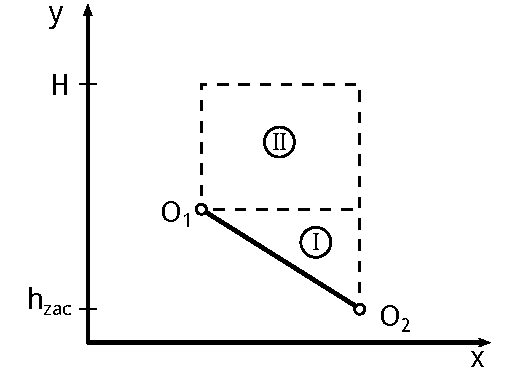
\includegraphics{slike/customChannel/odsek.pdf}\caption{Izbrani analizirani odsek struge} \label{fig:odsekStruge}
	\end{centering}
\end{figure}








% določitev ploščine posameznega kosa
Za vsak analizirani odsek dveh točk se določi najnižja točka odseka $T_z$, na sliki~\ref{fig:odsekStruge} označena kot točka $O_2$. Y koordinata točke $T_z$ nam predstavlja začetno višino odseka $h_{z}$. Od $h_z$ do končne višine gladine vode v strugi $H$ za vsak cm po višini določimo omočeni obod struge $P(h)$ in ploščino prečnega prereza odseka pod vodo $S(h)$.   Ravnina $g$ predstavlja gladino vode pri trenutni višini $h$, kar je prikazano na sliki~\ref{fig:custom_odsekDetajl}.


\begin{figure}[H]
	\begin{centering}
		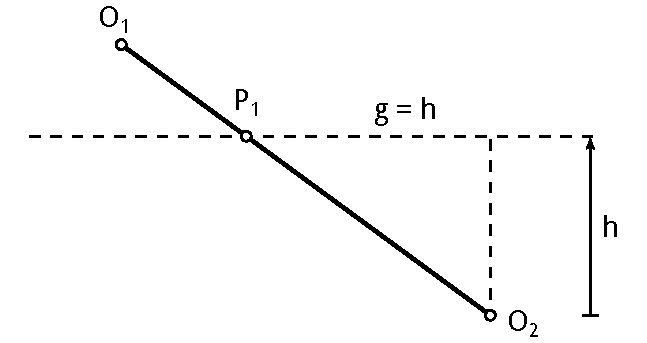
\includegraphics{slike/customChannel/odsek_detajl.pdf}\caption{Detajl izbranega odseka struge}\label{fig:custom_odsekDetajl}
	\end{centering}
\end{figure}



Omočeni obod struge vodotoka $P(h)$ in ploščina prečnega prereza struge vodotoka pod gladino vode $S(h)$ se glede na naklon funkcije $f(x)$, ki povezuje točki na robu analiziranega odseka izračuna na dva načina:

\begin{enumerate}

\item V primeru ko velja $\Delta y = 0$ je funkcija $f(x)$ med točkama trenutno analiziranega odseka vodoravna premica in dolžino omočenega oboda $P(h)$ ter ploščino prečnega prereza struge pod gladino vode $S(h)$ določimo kot:

\begin{ceqn}
\begin{align}
P(h)&= \Delta x\\
S(h)&= \Delta x \cdot h
\end{align}
\end{ceqn}


\item V primeru ko $\Delta y \neq 0$ ima funkcija $f(x)$ naklon $k \neq 0$. V tem primeru od začetka višine odseka $h_z$ do končne višine gladine vode v strugi vodotoka $H$ za vsak cm izračunamo presečišče $G$, funkcije $f(x)$ s horizontalno ravnino $g = h$, ki predstavlja gladino vode v strugi vodotoka. 


Ko imamo določeno presečišče $G$ gladine vode s funkcijo $f(x)$ med točkama analiziranega odseka, lahko izračunamo dolžino omočenega oboda struge odseka in ploščino lika, ki ga oklepajo funkcija odseka $f(x)$, navidezna gladina vode $g = h$ in najnižja točka odseka $T_z$ (na sliki \ref{fig:odsekStruge} označena z $O_2$). 



Način izračuna omočenega oboda struge vodotoka $P(h)$ in ploščine prečnega prereza pod gladino vode $S(h)$ je odvisen od pozicije presečišča $G$:


\begin{enumerate}
	\item V primeru da se presečišče $G$ izbranega odseka struge nahaja v območju med točkama $O_1$ in $O_2$, dolžino omočenega oboda določimo po Pitagorovem izreku kot:
	
	\begin{ceqn}
		\begin{align}
		P(h) = \sqrt{(T_{zx} - G_x(h))^{2} + (T_{zy} - G_y(h))^{2}}
		\end{align}
	\end{ceqn}
	
	
	Ploščino območja, ki ga oklepajo horizontalna ravnina $g$ s presečiščem $G$ in najnižjo točko odseka $T_z$ pa določimo kot ploščino trikotnika (območje I na sliki~\ref{fig:odsekStruge}) po formuli:
	
	\begin{ceqn}
		\begin{align}
		S(h) = \dfrac{|T_{zx} - G_x(h)| \cdot |T_{zy} - G_y(h)|}{2}
		\end{align}
	\end{ceqn}
	
	
	\item V primeru, da se presečišče $G$ nahaja izven območja točk $O_1$ in $O_2$ se dolžina omočenega oboda odseka izračuna kot razdalja med točkama $O_1$ in $O_2$ po Pitagorovem izreku:
	
	\begin{ceqn}
		\begin{align}
		P = \sqrt{ \Delta x^{2} + \Delta y^{2}}
		\end{align}
	\end{ceqn}
	
	Ploščina prečnega prereza struge vodotoka pod gladino vode analiziranega odseka $S(h)$ pa se določi kot seštevek ploščin območij I in II označenih na sliki \ref{fig:odsekStruge}.
	
	\begin{ceqn}
		\begin{align}
		S(h) = S_I + S_{II}(h)
		\end{align}
	\end{ceqn}
	
	Pri čemer sta $S_I$ in $S_{II}$ enaka:
	
		\begin{ceqn}
			\begin{align}
			S_I&= \bigg|\dfrac{ \Delta y \cdot  \Delta x}{2}\bigg|\\
			S_{II}(h)&= \bigg|\Delta x \cdot (h - y_1)\bigg|
			\end{align}
		\end{ceqn}
		
			
		
	\end{enumerate}

\end{enumerate}



Ko imamo za vsak cm višine gladine vode izračunan omočeni obod $P_m(h)$ odseka $m$ in ploščino prečnega prereza pod gladino vode $S_m(h)$ lahko določimo pretok vode skozi odsek struge vodotoka $Q_m(h)$. Pretok vode skozi odsek izračunamo po Manningovi enačbi opisani v poglavju \ref{sec:teorija_trapeznaMetoda}. Za vsak računani odsek $m$ moramo poznati tudi naklon struge vodotoka $I_m$ in  Manningov koeficient hrapavosti površine $ng_m$, ki se ju določi po postopkih opisanih v poglavju \ref{sec:teorija_pridobitevPodatkov}.


\begin{ceqn}
	\begin{align}
	Q_m(h) = \dfrac{\sqrt{I_m}}{ng_m} \cdot \dfrac{S_m(h)^{5/3}}{P_m(h)^{2/3}}
	\end{align}
\end{ceqn}


Posamezne pretoke odsekov po višinah medsebojno seštejemo in dobimo končne vrednosti pretokov $Q$ v odvisnosti od višine gladine vode v strugi vodotoka, kar je shematično prikazano na sliki~\ref{fig:customChannel_sestevek}:

\begin{ceqn}
	\begin{align}
	%Q(h) = Q_1(h) + Q_2(h) + Q_3(h) + ... + Q_{n-1}(h) + Q_n(h)
	Q(h) = \sum_{1}^{n} Q_n(h)
	\end{align}
\end{ceqn}


\begin{figure}[ht!]
	\begin{centering}
		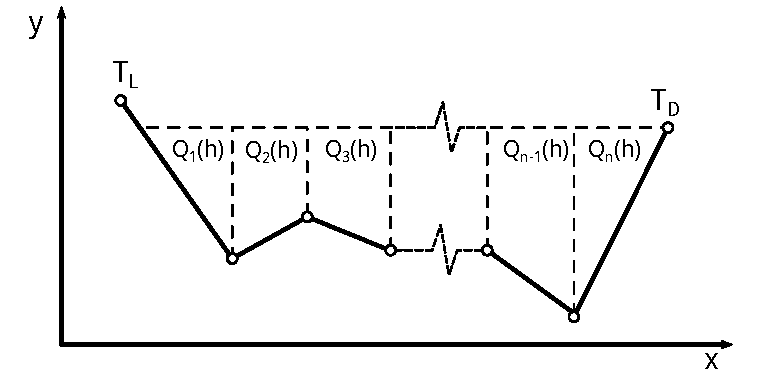
\includegraphics{slike/customChannel/sestevekPretokov.pdf}
		\caption{Prikaz seštevka pretokov po odsekih}\label{fig:customChannel_sestevek}
	\end{centering}
\end{figure}



S tem postopkom smo določili vse točke, ki določajo konsumpcijsko krivuljo $h(Q)$ za izbrano strugo poljubne oblike.


\newpage

\section{Izračun proizvodnje električne energije}
Za določitev proizvodnje električne energije potrebujemo podatek o razliki med koto zgornje vode t.j. vode v rezervoarju in koto spodnje vode t.j. vode, ki teče skozi turbine hidroelektrarne. Ker računamo proizvodnjo električne energije za pretočne hidroelektrarne predpostavimo, da je kota zgornje vode konstantna na višini $H_z$.

\begin{figure}[ht!]
	\begin{centering}
		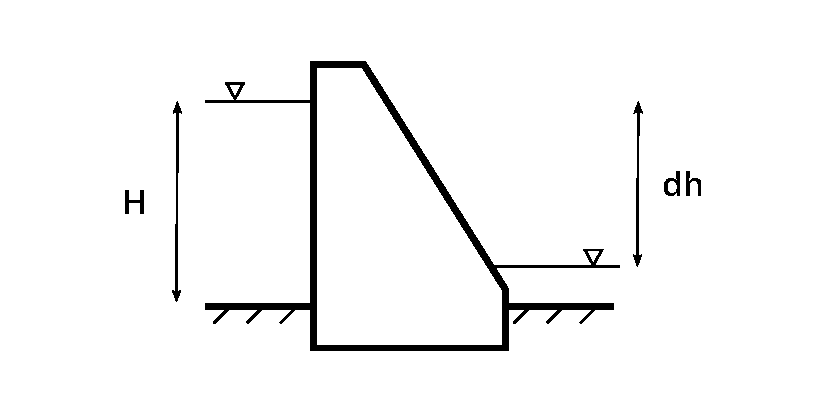
\includegraphics{slike/electricityProduction/powerplant_crossSection.pdf}
		\caption{Shema prečnega prereza hidroelektrarne}
	\end{centering}
\end{figure}

 Koto spodnje vode $H_s$ določimo iz prej izračunane konsumpcijske krivulje iz katere odčitamo višino gladine vode v strugi za dani povprečni mesečni pretok ki teče skozi turbine hidroelektrarne. V primeru da se pretok skozi turbine hidroelektrarne nahaja med dvema točkama pretokov v konsumpcijski krivulji, iskano višino spodnje vode določimo z linearno interpolacijo med znanima izračunanima točkama na grafu konsumpcijske krivulje.


Višinsko razliko med koto zgornje in spodnje vode določimo po spodnji enačbi:

\begin{ceqn}
\begin{align}
dh = H_z - H_s
\end{align}
\end{ceqn}

Moč hidroelektrarne izračunamo po enačbi:

\begin{ceqn}
\begin{align}
P = \eta \cdot \dfrac{g \cdot \rho_v}{1000} \cdot Q_t \cdot dh \label{eq:mocHidroelektrarne}
\end{align}
\end{ceqn}

Pri čemer so:
\begin{table}[htb!]
	\begin{tabular}{r|p{10cm}}
		P & moč [$kW$]\\
		$\eta$ & izkoristek turbine [\%]\\
		g & gravitacijska konstanta $\left[9,81~\dfrac{m}{s^{2}}\right]$ \\
		$\rho_v$&gostota vode $\left[\dfrac{1000 kg}{m^3}\right]$\\
		$Q_t$ & pretok skozi turbine hidroelektrarne $\left[m^{3}/s \right]$\\
		dh & razlika višin med koto spodnje in koto zgornje vode [$m$]
	\end{tabular}
\end{table}



% opis kako izračunamo povprečno moč hidroelektrarne:
% 1. kako določimo Q, 
% 2. kje dobimo podatke o pretokih (analiza hidroloških podatkov)

Izkoristek turbin hidroelektrarne je načeloma odvisen od pretoka vode skozi turbine, vendar lahko to lastnost turbin za potrebe ocene proizvodnje električne energije zanemarimo. Pretok vode skozi turbine hidroelektrarne $Q_t$ je odvisen od parametrov hidroelektrarne in pretoka vodotoka. $Q_t$ se določi glede na spodnje pogoje:

\begin{ceqn}
	\begin{align}
	Q_t = \begin{cases}
	0, &Q < Q_{min}\\
	Q, &Q_{min} < Q < Q_{max}\\
	Q_{max}, &Q_{max}< Q < Q_{teh}\\
	0, &Q > Q_{teh}\\
	\end{cases}
	\end{align}
\end{ceqn}

Pri čemer so:
\begin{table}[htb!]
	\begin{tabular}{r|p{10cm}}
		$Q$ & Pretok vodotoka $\left[m^3/s \right]$\\
		$Q_{min}$ & biološki minimum pretoka vodotoka $\left[m^3/s \right]$ \\
		$Q_{max}$ & instalirani pretok $\left[m^3/s \right]$ \\
		$Q_{teh}$ & tehnični maksimum pretoka hidroelektrarne $\left[m^3/s \right]$ \\
	\end{tabular}
\end{table}

%TODO: fix this part
V primeru, ko je pretok vodotoka manjši kot biološki minimum, ki se zahteva zato, da reka ne presahne, se vsa voda preliva skozi prelivna polja hidroelektrarne in do proizvodnje električne energije ne pride. V primeru poplav, ko je pretok vodotoka večji od tehničnega maksimuma pretoka hidroelektrarne se vsa voda preliva preko jezu in hidroelektrarna prav tako ne proizvaja električne energije. V vseh ostalih primerih pretokov vodotoka, pa je pretok skozi turbine kar enak pretoku vodotoka z maksimalnim pretokom pri $Q_t = Q_{max}$. Maksimalni pretok $Q_{max}$ se določi na podlagi izbranih turbin hidroelektrarne, določenih s pomočjo krivulje trajanja.


%-----

Za določitev povprečne mesečne proizvodnje električne energije potrebujemo znano povprečno mesečno moč hidroelektrarne  $\overline{P}$. Povprečno mesečno moč hidroelektrarne izračunamo s povprečjem dnevnih moči hidroelektrarne za iskani mesec po enačbi~\ref{eq:mocHidroelektrarne}. Podatke o povprečnih mesečnih pretokih pridobimo iz rezultatov analize hidrološkega niza podatkov opisane v poglavju~\ref{sec:teorija_hidrogramObdobja}. Za vsak mesec izračunamo povprečno moč hidroelektrarne po spodnji enačbi, pri čemer je $n$ število dni v mesecu. 



\begin{ceqn}
\begin{align}
\overline{P} = \dfrac{P_1 + P_2 + P_3 + ... + P_{n-1} + P_n}{n}
\end{align}
\end{ceqn}



Povprečno mesečno proizvodnjo električne energije n-tega meseca izračunamo po naslednji enačbi:

\begin{ceqn}
\begin{align}
E_n = \dfrac{24 \cdot \overline{P} \cdot d}{1000}
\end{align}
\end{ceqn}

Pri čemer so:
\begin{table}[htb!]
\begin{tabular}{r|p{10cm}}
	$E_n$ & povprečna mesečna proizvedena električna energija [$MWh$]\\
	$\overline{P}$ & povprečna moč v mesecu [$kW$]\\
	$d$ & število dni v mesecu \\
\end{tabular}
\end{table}


Povprečno letno proizvodnjo električne energije se izračuna s seštevkom vseh povprečnih mesečnih proizvodenj:
\begin{ceqn}
	\begin{align}
	E_{leto} =  \dfrac{E_{1} + E_{2} + E_{3} + ... + E_{10} + E_{11} + E_{12}}{1000} ~[GWh]
	\end{align}
\end{ceqn}

